\documentclass{bioinfo}
\usepackage{subfigure}
\usepackage{amsmath}

\usepackage{color,soul}  % for markup
\setul{1ex}{0.8ex}
\definecolor{orange}{rgb}{1,0.5,0}
\newcommand{\marked}[1]{\hl{#1}}
\newcommand{\comment}[1]{\hl{\bf FIXME! #1}}

\copyrightyear{2012}
\pubyear{2012}

\begin{document}
\firstpage{1}
\title[CTLmapping]{CTL mapping - The added value from segregating correlation}

\author[Arends \emph{et al.}]{
  Danny Arends\,$^{1,\footnote{to whom correspondence should be addressed}}$,
  Pjotr Prins\,$^{1,2}$
  and Ritsert C. Jansen\,$^{1}$
}
\address{
  $^{1}$Groningen \hl{Bio-informatics} Centre, University of Groningen, Groningen, The Netherlands.
  $^{2}$Laboratory of Nematology, Wageningen University, The Netherlands.
}
\history{Received on XXXXX; revised on XXXXX; accepted on XXXXX}
\editor{Associate Editor: XXXXX}
\maketitle

\comment{Title is too cute, and looks too much like an earlier paper;
also should be more descriptive}

\comment{3x Groningen in address. And does that dash belong there?}

\begin{abstract}
  \section{Summary:}
  
  % Summary moet 1 of 2 zinnen zijn! Zoiets beter?
 
  Mapping of correlated traits loci (CTL) to the genome potentially
  allows the detection of genetic regulation of traits by tracking
  correlation differences at genetic marker locations. CTL can be
  combined with quantitative trait loci (QTL) in regulatory network
  reconstruction.
  
  %  , in almost the same way as QTL mapping associates genetic
  %  markers with differences in expression.  <- als je dit zegt is
  %  het niet zo nieuw meer ;)
  
  % We use CTL mapping to reconstruct underlying genetic architecture, and provide insight 
  % into regulation of (gene) expression. CTL information in combination with classical QTL 
  % information leads to a more detailed insight into the genetic architecture underlying 
  % complex traits. CTL mapping 

  \section{Availability:}

  The software is available under the terms of GNU General Public License, version 3
  (\href{http://www.r-project.org/Licenses/GPL-3}{www.r-project.org/Licenses/GPL-3}).
  \section{Availability:}
  Software, documentation and source code are available at request.
  \section{Contact:} 
  \href{Danny.Arends\hl{@Gmail.com}}{Danny.Arends@\hl{Gmail.com}}
\end{abstract}

\comment{Use university E-mail}

\comment{License: BSD license is preferred these days}

\comment{Availability: Bioinformatics Journal wants open source software only,
availability should reflect that - i.e. a github.org repo. They won't
like your option ;)}

\section{Introduction}
  Genetical genomics experiments have shown that gene expression variation can be mapped to 
  genetic variation \cite{Jansen:2001}. Quantitative Trait Locus (QTL) mapping of a 
  gene identifies regions in the genome for which different genotypes lead to differential 
  expression level of the gene. This QTL mapping can be done on all molecular levels including, 
  gene expression (eQTL), protein abundance (pQTL) and metabolites (mQTL).
  
  We present Correlated Traits Locus (CTL) mapping as a comparable method to QTL mapping.
  CTL unlike QTL links differences in correlation to genetic variation, i.e. to identify regions in the 
  genome for which one genotype value leads to correlated expression between a trait and  
  other traits, while the other genotype doesn't show this correlation. CTL exploits the fact that 
  any QTL will be the result of either direct induced variation or indirect variation. The latter is 
  visible as correlation differences among individuals carrying different genotypes.
  
  We merge information coming from CTL and QTL to reveal underlying genetic architecture, which 
  would remain hidden when using only classical QTL information.

\section{Methodology}
  Choose a trait to subject to CTL analysis, this can be your favourite gene, 
  protein, metabolite or classical trait.

  Split the population at a genetic marker in two groups (A and B). Calculate the correlation 
  between our trait of interest and other traits. Then calculate the CTL score by taking the 
  squared difference between A and B.

  \begin{figure*}[ht]
    \begin{center}
    \vspace{-0.2cm}
    \hspace{-1.3cm}
    \subfigure[CTL profiles]{
      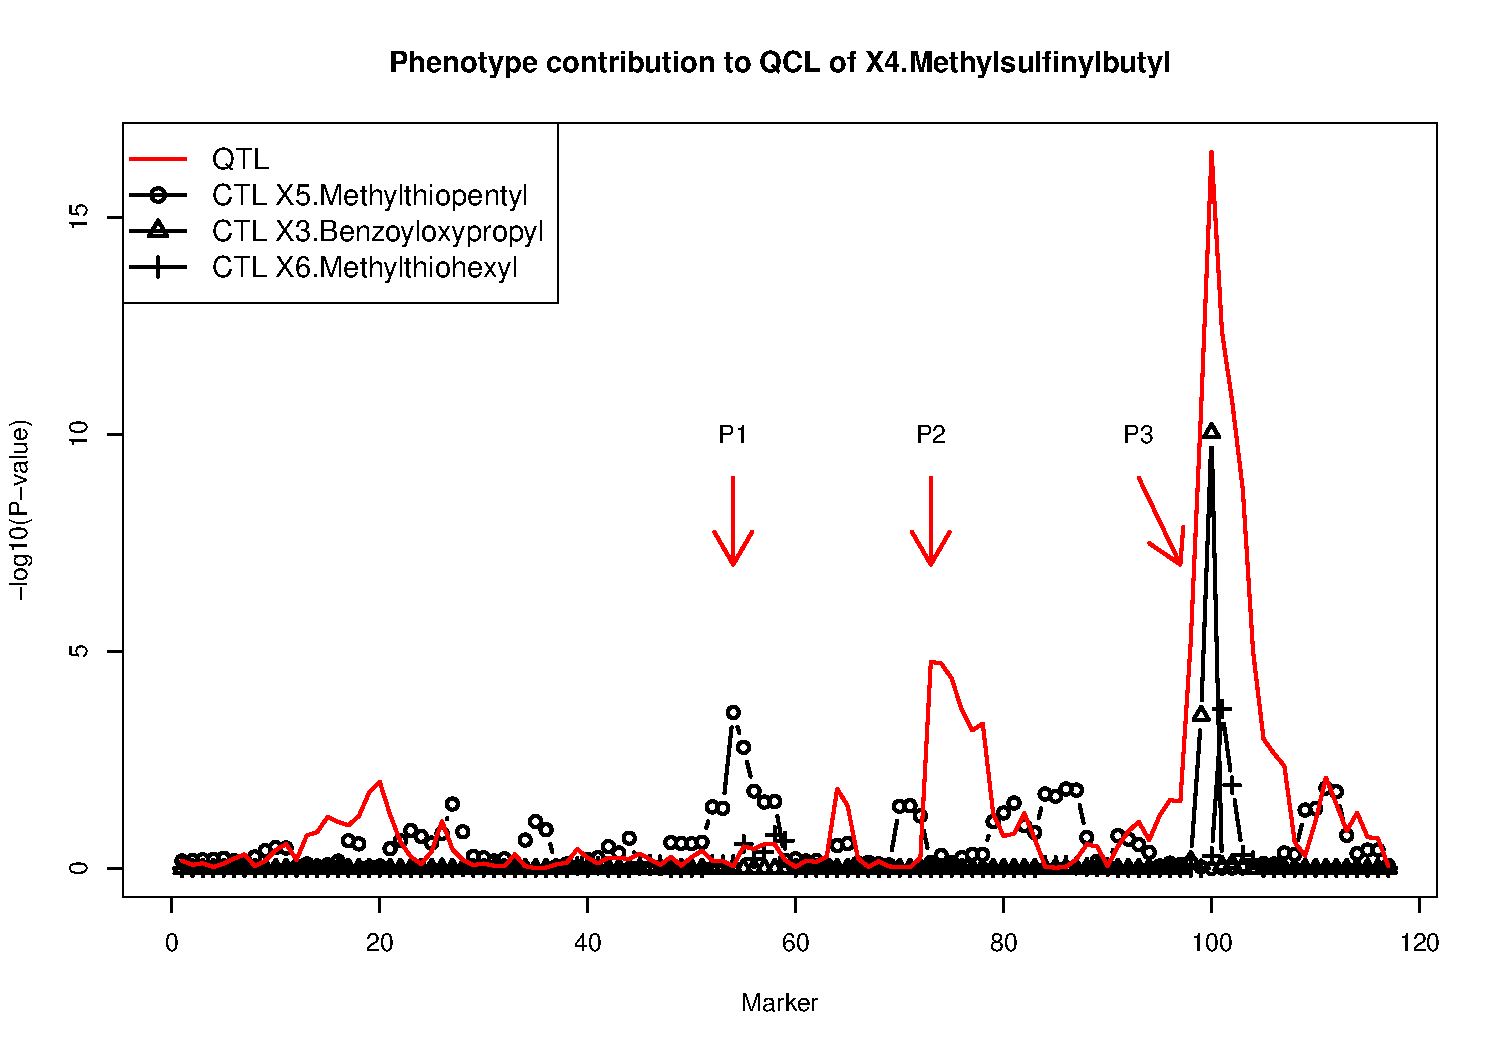
\includegraphics[keepaspectratio,scale=.3]{img/ctl_qtl.eps}
      \label{subfiga}
    }
    \hspace{0.3cm}
    \subfigure[Traits x Traits interaction matrix]{
      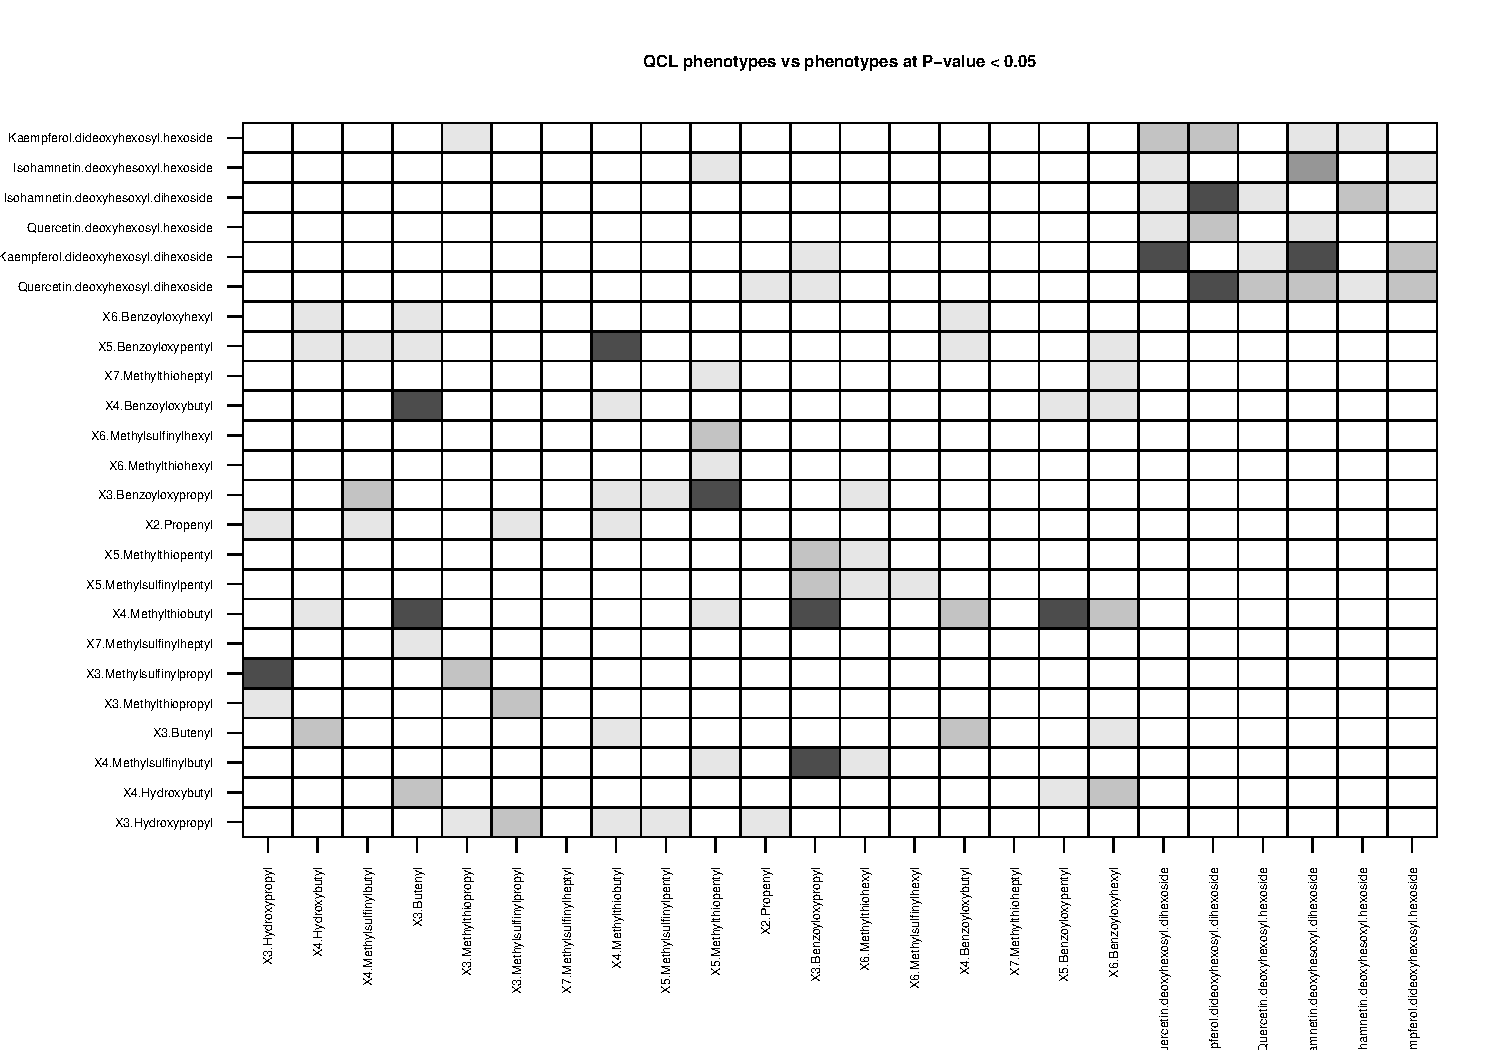
\includegraphics[keepaspectratio,scale=.3]{img/ctl_pxp.eps}
      \label{subfigb}
    }
    \hspace{0.3cm}
    \subfigure[Reconstructed network]{
      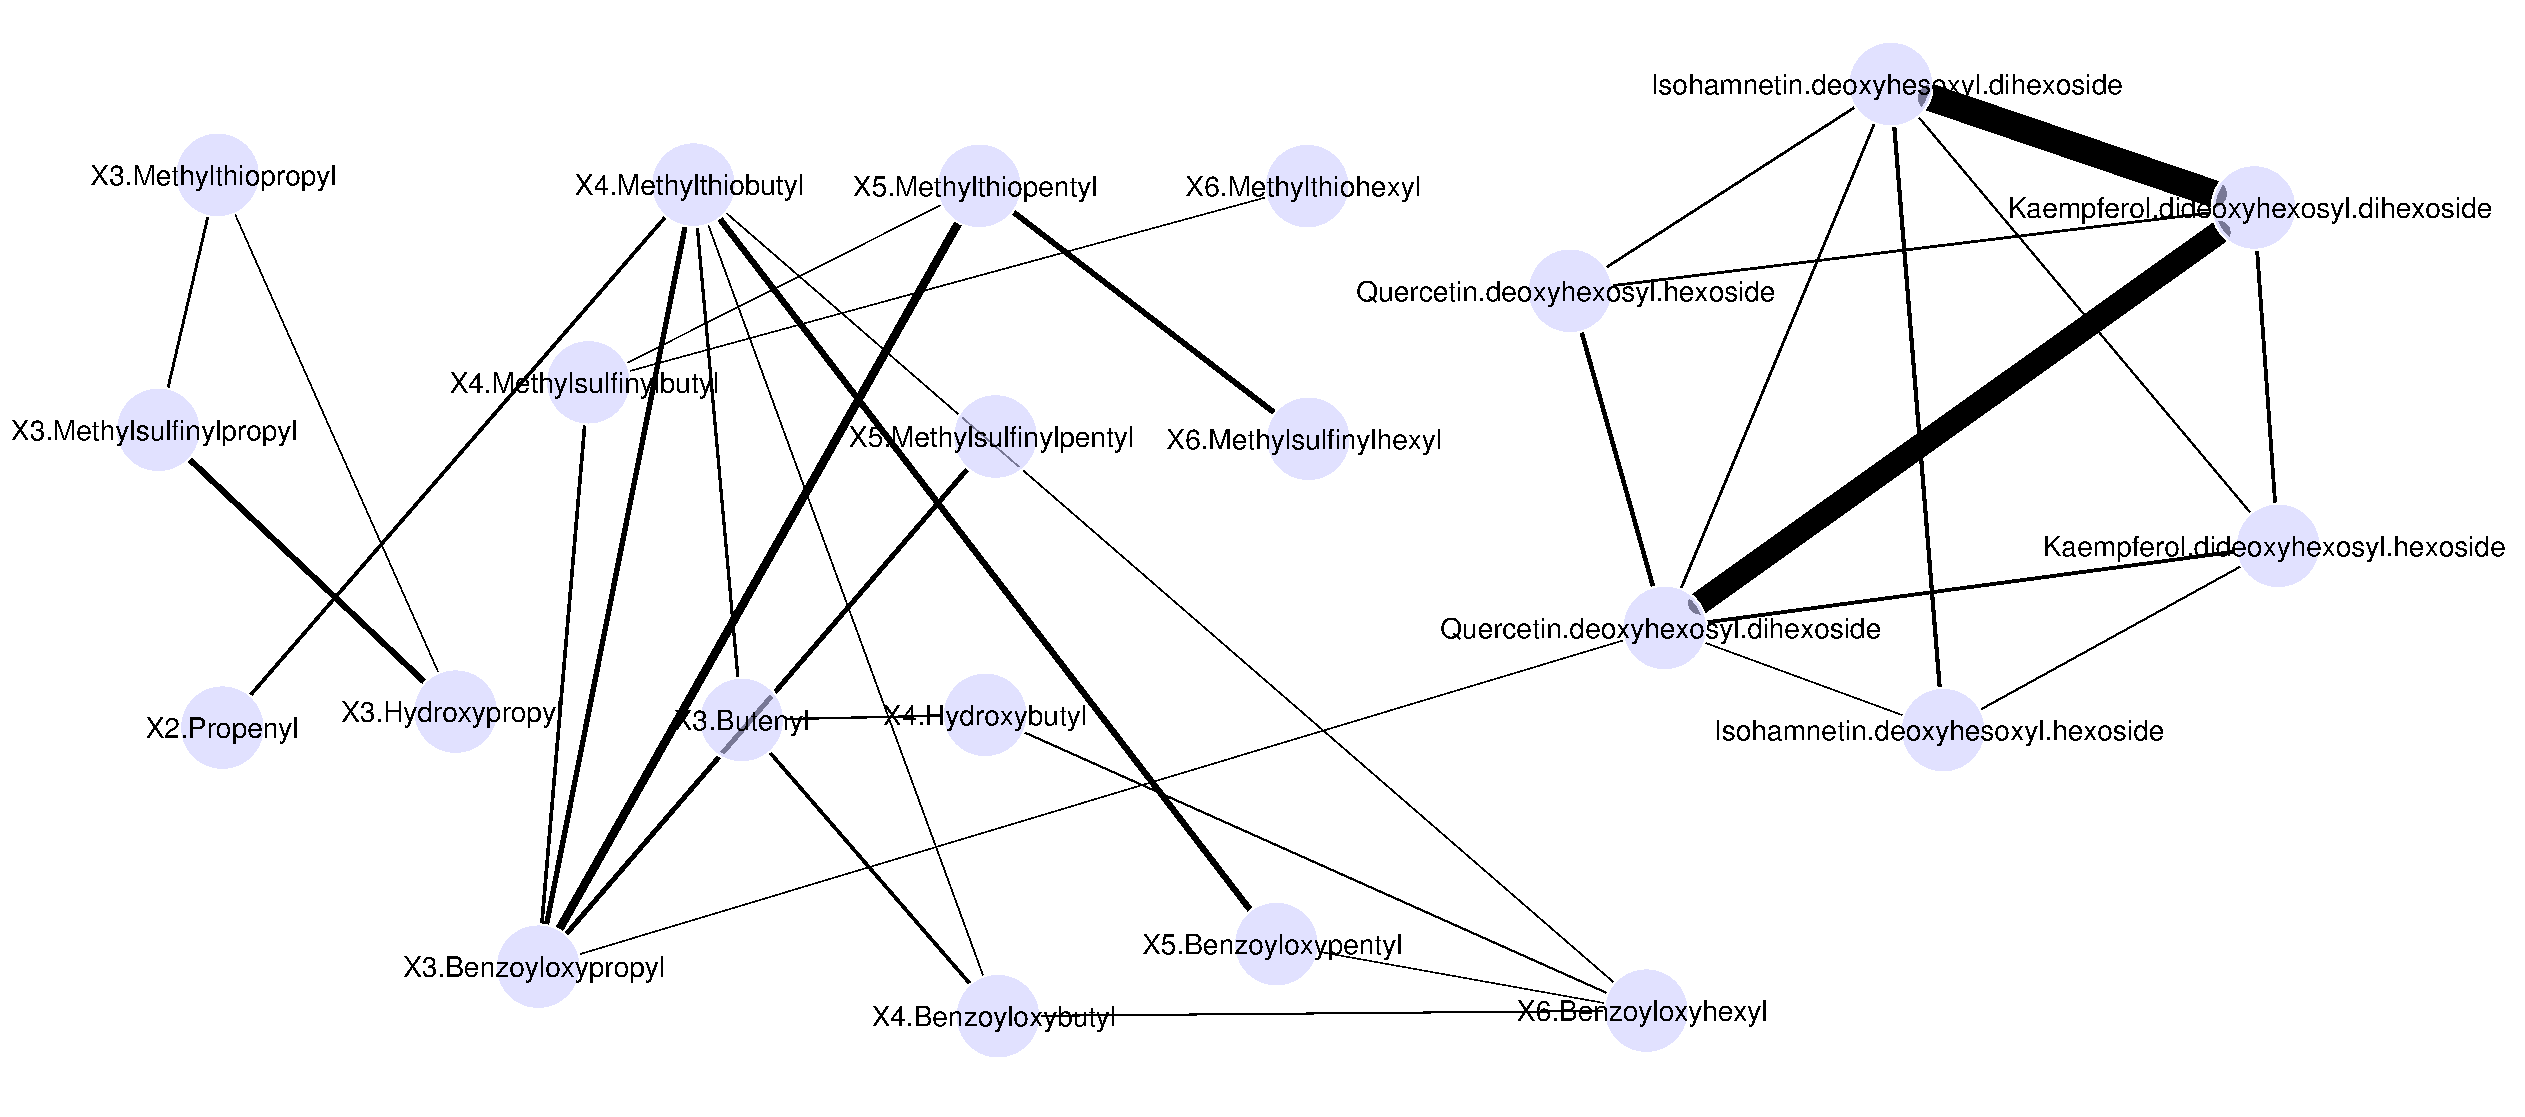
\includegraphics[keepaspectratio,scale=.3]{img/ctl_net.eps}
      \label{subfigc}
    }
  \end{center}
  \begin{minipage}{7in}
  \label{newplots}
  \vspace{-0.7cm}
  \caption[Plots]{
  {\emph {\bf a}}: Example CTL + QTL profiles. Seen are the QTL profile on top of the CTL profile. 
  The first peak is a CTL, we don't observe a QTL for this location.
  The second peak is a QTL peek, with no underlying CTL. \hl{You
  should explain P1,P2 and P3 in the caption too! A figure should be
  read on its own} 
  {\emph {\bf b}}: Traits x Traits interaction matrix (TxT matrix). Information obtained using CTL mapping, 
  showing for each trait the significance of the difference in correlation to all other traits. This 
  matrix can be transformed into .sif file to generate a network image. 
  {\emph {\bf c}}:  Reconstructed network, this shows the same information as the TxT matrix only in a more accessible way, we visualized our 
  network using cytoscape, the width of the line is the maximum interaction evidence.
 }
\end{minipage}
\vspace{-0.5cm}
\end{figure*}

\emph{ {\bf Significance testing}}
  Comparing CTL profiles to QTL profiles CTL scores need to be converted to LOD scores. Significance 
  of CTL is assessed by using permutations, in each round the link between genotype and 
  trait is broken, by redistributing at random genotypes amongst individuals not 
  allowing for duplicates. When we observe CTL scores in real data which are higher than any 
  CTL score obtained during permutation a generalized Pareto distribution (GPD) is used to 
  estimate the extreme tail of the distribution \cite{Knijnenburg:2009}, to get likelihood estimates for the 
  extreme scores observed.

\emph{ {\bf Materials}}
  Metabolite data from an \emph{A. Thaliana} Landsberg erecta (Ler) and Cape Verde Islands (Cvi) 
  dataset from R/qtl, 24 characterized metabolites which are the products of chain elongation. 
  There are 162 recombinant inbred lines genotyped at 117 markers on 5 chromosomes. Additional 
  details about the experimental settings are available in the original paper \cite{Keurentjes:2006,AlonsoBlanco:1998}
\vspace{-0.6cm}
\section{FEATURES}
  CTL mapping was performed and a per trait CTL thresholds of $P < 0.001$ was 
  determined by using 15,000 permutations.
  When combining CTL and QTL information, we observe:\\
  1) Additional CTL found, where no QTL was present (Fig \ref{subfiga} - P1). Loss of variation in the genes 
  underneath the CTL are not causing variation differences in the observed trait, CTL is able to 
  detect the differences in correlation.\\
  2) QTL with no CTL (Fig \ref{subfiga} - P2), we interpret this as the source of the variation. Analysis in this way of 
  all 24 Single trait CTL profiles combined with their QTL profiles allows us to reconstruct the 
  source of natural variation and follow it down the network.
  3) CTL co-localized with QTL, in this situation CTL gives a detailed view of which traits 
  are contributing variation to the observed QTL  (Fig \ref{subfiga} - P3).\\
  
  Information obtained by CTL mapping is shown in the trait to trait interaction matrix (Fig. \ref{subfigb}).

\emph{ {\bf Network reconstruction}}
  Using the information from CTL and QTL we are able to draw arrows between traits, reconstruct the interaction 
  network amongst the 24 metabolities in Arabidopsis (Fig. \ref{subfigc}). We observe that our network is 
  composed of 2 parts which seem connected only by a just significant CTL from X3.Benzoyloxypropyl to 
  Quercetin.deoxyhexosyl.dihexoside.

\section{Conclusion}
  Microarray experiments have identified genes differentially expressed between various 
  conditions, or groups of genes coexpressed across samples. Genetical genomics screens 
  are carried out to map differential expression to genetic variation. Screening 
  the genome for genotype combinations for which there is differential expression is 
  a successful strategy when mapping Mendelian traits. 
  
  Results on complex traits however have been less then satisfactory with only small 
  amounts of heritability explained by individuals loci. CTL mapping 'borrows'
  information from all traits in the analysis, and extracts trait to trait 
   information.
 
  Furthermore CTLs seem to 'transfer' from trait to traits in a stabile 
  fashion, allowing reconstructing of genetic architecture. CTL combined with QTL 
  data identify gene transcript introducing variation (by absense), while co-localizing 
  with QTL affected by upstream variation.

\paragraph{Funding\textcolon}
The Centre for BioSystems Genomics (CBSG) and the Netherlands Consortium of Systems 
Biology (NCSB), both of which are part of the Netherlands Genomics Initiative / 
Netherlands Organisation for Scientific Research [to DA]; the EU 7th Framework 
Programme under the Research Project PANACEA [222936 to R.J.].
\vspace{-0.7cm}
\bibliographystyle{natbib}
\bibliography{document}
\end{document}
